\documentclass[]{article}
\usepackage{lmodern}
\usepackage{amssymb,amsmath}
\usepackage{ifxetex,ifluatex}
\usepackage{fixltx2e} % provides \textsubscript
\ifnum 0\ifxetex 1\fi\ifluatex 1\fi=0 % if pdftex
  \usepackage[T1]{fontenc}
  \usepackage[utf8]{inputenc}
\else % if luatex or xelatex
  \ifxetex
    \usepackage{mathspec}
  \else
    \usepackage{fontspec}
  \fi
  \defaultfontfeatures{Ligatures=TeX,Scale=MatchLowercase}
\fi
% use upquote if available, for straight quotes in verbatim environments
\IfFileExists{upquote.sty}{\usepackage{upquote}}{}
% use microtype if available
\IfFileExists{microtype.sty}{%
\usepackage{microtype}
\UseMicrotypeSet[protrusion]{basicmath} % disable protrusion for tt fonts
}{}
\usepackage[margin=1in]{geometry}
\usepackage{hyperref}
\hypersetup{unicode=true,
            pdftitle={Homework 3},
            pdfauthor={Christophe Hunt},
            pdfborder={0 0 0},
            breaklinks=true}
\urlstyle{same}  % don't use monospace font for urls
\usepackage{color}
\usepackage{fancyvrb}
\newcommand{\VerbBar}{|}
\newcommand{\VERB}{\Verb[commandchars=\\\{\}]}
\DefineVerbatimEnvironment{Highlighting}{Verbatim}{commandchars=\\\{\}}
% Add ',fontsize=\small' for more characters per line
\usepackage{framed}
\definecolor{shadecolor}{RGB}{248,248,248}
\newenvironment{Shaded}{\begin{snugshade}}{\end{snugshade}}
\newcommand{\KeywordTok}[1]{\textcolor[rgb]{0.13,0.29,0.53}{\textbf{{#1}}}}
\newcommand{\DataTypeTok}[1]{\textcolor[rgb]{0.13,0.29,0.53}{{#1}}}
\newcommand{\DecValTok}[1]{\textcolor[rgb]{0.00,0.00,0.81}{{#1}}}
\newcommand{\BaseNTok}[1]{\textcolor[rgb]{0.00,0.00,0.81}{{#1}}}
\newcommand{\FloatTok}[1]{\textcolor[rgb]{0.00,0.00,0.81}{{#1}}}
\newcommand{\ConstantTok}[1]{\textcolor[rgb]{0.00,0.00,0.00}{{#1}}}
\newcommand{\CharTok}[1]{\textcolor[rgb]{0.31,0.60,0.02}{{#1}}}
\newcommand{\SpecialCharTok}[1]{\textcolor[rgb]{0.00,0.00,0.00}{{#1}}}
\newcommand{\StringTok}[1]{\textcolor[rgb]{0.31,0.60,0.02}{{#1}}}
\newcommand{\VerbatimStringTok}[1]{\textcolor[rgb]{0.31,0.60,0.02}{{#1}}}
\newcommand{\SpecialStringTok}[1]{\textcolor[rgb]{0.31,0.60,0.02}{{#1}}}
\newcommand{\ImportTok}[1]{{#1}}
\newcommand{\CommentTok}[1]{\textcolor[rgb]{0.56,0.35,0.01}{\textit{{#1}}}}
\newcommand{\DocumentationTok}[1]{\textcolor[rgb]{0.56,0.35,0.01}{\textbf{\textit{{#1}}}}}
\newcommand{\AnnotationTok}[1]{\textcolor[rgb]{0.56,0.35,0.01}{\textbf{\textit{{#1}}}}}
\newcommand{\CommentVarTok}[1]{\textcolor[rgb]{0.56,0.35,0.01}{\textbf{\textit{{#1}}}}}
\newcommand{\OtherTok}[1]{\textcolor[rgb]{0.56,0.35,0.01}{{#1}}}
\newcommand{\FunctionTok}[1]{\textcolor[rgb]{0.00,0.00,0.00}{{#1}}}
\newcommand{\VariableTok}[1]{\textcolor[rgb]{0.00,0.00,0.00}{{#1}}}
\newcommand{\ControlFlowTok}[1]{\textcolor[rgb]{0.13,0.29,0.53}{\textbf{{#1}}}}
\newcommand{\OperatorTok}[1]{\textcolor[rgb]{0.81,0.36,0.00}{\textbf{{#1}}}}
\newcommand{\BuiltInTok}[1]{{#1}}
\newcommand{\ExtensionTok}[1]{{#1}}
\newcommand{\PreprocessorTok}[1]{\textcolor[rgb]{0.56,0.35,0.01}{\textit{{#1}}}}
\newcommand{\AttributeTok}[1]{\textcolor[rgb]{0.77,0.63,0.00}{{#1}}}
\newcommand{\RegionMarkerTok}[1]{{#1}}
\newcommand{\InformationTok}[1]{\textcolor[rgb]{0.56,0.35,0.01}{\textbf{\textit{{#1}}}}}
\newcommand{\WarningTok}[1]{\textcolor[rgb]{0.56,0.35,0.01}{\textbf{\textit{{#1}}}}}
\newcommand{\AlertTok}[1]{\textcolor[rgb]{0.94,0.16,0.16}{{#1}}}
\newcommand{\ErrorTok}[1]{\textcolor[rgb]{0.64,0.00,0.00}{\textbf{{#1}}}}
\newcommand{\NormalTok}[1]{{#1}}
\usepackage{graphicx,grffile}
\makeatletter
\def\maxwidth{\ifdim\Gin@nat@width>\linewidth\linewidth\else\Gin@nat@width\fi}
\def\maxheight{\ifdim\Gin@nat@height>\textheight\textheight\else\Gin@nat@height\fi}
\makeatother
% Scale images if necessary, so that they will not overflow the page
% margins by default, and it is still possible to overwrite the defaults
% using explicit options in \includegraphics[width, height, ...]{}
\setkeys{Gin}{width=\maxwidth,height=\maxheight,keepaspectratio}
\IfFileExists{parskip.sty}{%
\usepackage{parskip}
}{% else
\setlength{\parindent}{0pt}
\setlength{\parskip}{6pt plus 2pt minus 1pt}
}
\setlength{\emergencystretch}{3em}  % prevent overfull lines
\providecommand{\tightlist}{%
  \setlength{\itemsep}{0pt}\setlength{\parskip}{0pt}}
\setcounter{secnumdepth}{5}
% Redefines (sub)paragraphs to behave more like sections
\ifx\paragraph\undefined\else
\let\oldparagraph\paragraph
\renewcommand{\paragraph}[1]{\oldparagraph{#1}\mbox{}}
\fi
\ifx\subparagraph\undefined\else
\let\oldsubparagraph\subparagraph
\renewcommand{\subparagraph}[1]{\oldsubparagraph{#1}\mbox{}}
\fi

%%% Use protect on footnotes to avoid problems with footnotes in titles
\let\rmarkdownfootnote\footnote%
\def\footnote{\protect\rmarkdownfootnote}

%%% Change title format to be more compact
\usepackage{titling}

% Create subtitle command for use in maketitle
\newcommand{\subtitle}[1]{
  \posttitle{
    \begin{center}\large#1\end{center}
    }
}

\setlength{\droptitle}{-2em}
  \title{Homework 3}
  \pretitle{\vspace{\droptitle}\centering\huge}
  \posttitle{\par}
  \author{Christophe Hunt}
  \preauthor{\centering\large\emph}
  \postauthor{\par}
  \predate{\centering\large\emph}
  \postdate{\par}
  \date{February 18, 2017}

\usepackage{relsize}
\usepackage{setspace}
\usepackage{amsmath,amsfonts,amsthm}
\usepackage[sfdefault]{roboto}
\usepackage[T1]{fontenc}
\usepackage{float}

\begin{document}
\maketitle

{
\setcounter{tocdepth}{2}
\tableofcontents
}
\newpage

\section{Problem : Page 113: 2}\label{problem-page-113-2}

The following table gives the elongation \(e\) in inches (in./in.) for a
given stress \(S\) on a steel wire measured in pounds per square inch
(lb/in.\(^2\)). Test the models \(e = c_1S\) by plotting the data.
Estimate \(c_1\) graphically.

\begin{table}[!htbp]
\centering
\caption{}
\label{my-label}
\begin{tabular}{l|lllllllllll}
$S(x10^{-3})$ & 5 & 10 & 20 & 30 & 40  & 50  & 60  & 70  & 80  & 90  & 100 \\ \hline
$e(x10^5)$    & 0 & 19 & 57 & 94 & 134 & 173 & 216 & 256 & 297 & 343 & 390 
\end{tabular}
\end{table}

\begin{Shaded}
\begin{Highlighting}[]
\KeywordTok{library}\NormalTok{(ggplot2)}
\NormalTok{S <-}\StringTok{ }\KeywordTok{c}\NormalTok{(}\DecValTok{5}\NormalTok{,}\DecValTok{10}\NormalTok{,}\DecValTok{20}\NormalTok{,}\DecValTok{30}\NormalTok{,}\DecValTok{40}\NormalTok{,}\DecValTok{50}\NormalTok{,}\DecValTok{60}\NormalTok{,}\DecValTok{70}\NormalTok{,}\DecValTok{80}\NormalTok{,}\DecValTok{90}\NormalTok{,}\DecValTok{100}\NormalTok{)}
\NormalTok{e <-}\StringTok{ }\KeywordTok{c}\NormalTok{(}\DecValTok{0}\NormalTok{,}\DecValTok{19}\NormalTok{,}\DecValTok{57}\NormalTok{,}\DecValTok{94}\NormalTok{,}\DecValTok{134}\NormalTok{,}\DecValTok{173}\NormalTok{,}\DecValTok{216}\NormalTok{,}\DecValTok{256}\NormalTok{,}\DecValTok{297}\NormalTok{,}\DecValTok{343}\NormalTok{,}\DecValTok{390}\NormalTok{)}
\KeywordTok{ggplot}\NormalTok{(}\DataTypeTok{data =} \KeywordTok{as.data.frame}\NormalTok{(}\KeywordTok{cbind}\NormalTok{(S,e)), }\KeywordTok{aes}\NormalTok{(}\DataTypeTok{x =} \NormalTok{S, }\DataTypeTok{y =} \NormalTok{e)) +}\StringTok{ }
\StringTok{  }\KeywordTok{geom_point}\NormalTok{() +}
\StringTok{  }\KeywordTok{geom_abline}\NormalTok{(}\DataTypeTok{slope =} \FloatTok{3.6}\NormalTok{, }\DataTypeTok{color =} \StringTok{'blue'}\NormalTok{) +}\StringTok{ }
\StringTok{  }\KeywordTok{geom_abline}\NormalTok{(}\DataTypeTok{intercept =} \NormalTok{-}\DecValTok{20}\NormalTok{, }\DataTypeTok{slope =} \DecValTok{4}\NormalTok{, }\DataTypeTok{color =} \StringTok{'red'}\NormalTok{)}
\end{Highlighting}
\end{Shaded}

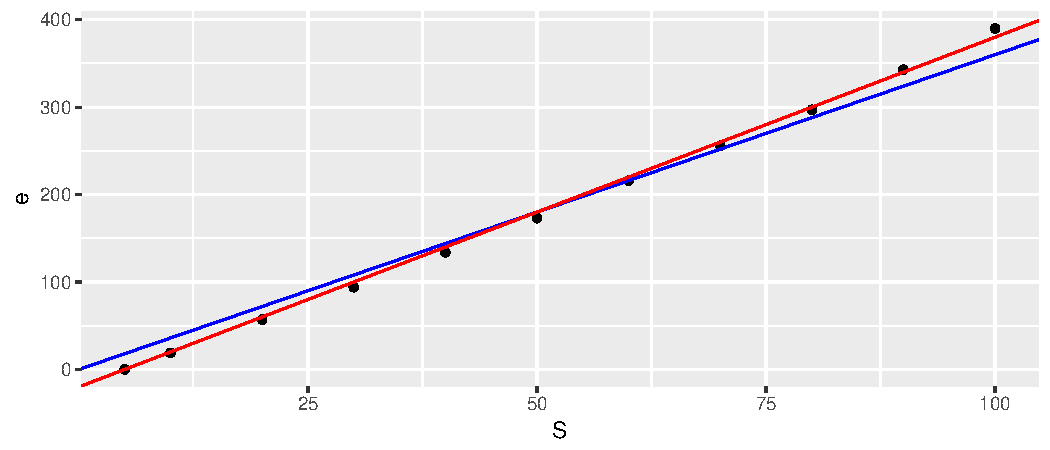
\includegraphics{Christophe_Hunt_hw3_files/figure-latex/unnamed-chunk-1-1.pdf}

\begin{quote}
Above is the graph of the elongation \$e\% versus stress S x
10\^{}\{-1\}. By eyeballing the results of several plots we can give the
estimate of \textasciitilde{}3.6 for \(c_1\) for the model \(e = c_1S\)
(this is the blue line). However, do see a much better fit with
\textasciitilde{}4 for \(c_1\), if we provide an intercept of -20. These
are simply best guesses.
\end{quote}

\newpage

\section{Problem : Page 121: 2.a}\label{problem-page-121-2.a}

For each of the following data sets, formulate the mathematical model
that minimizes the largest deviation between the data and the line y =
ax + b. If a computer is available, solve for the estimates of a and b.

\begin{table}[!htbp]
\centering
\caption{}
\label{my-label}
\begin{tabular}{l|llllll}
x & 1   & 2.3 & 3.7 & 4.2 & 6.1 & 7.0 \\ \hline
y & 3.6 & 3.0 & 3.2 & 5.1 & 5.3 & 6.8  
\end{tabular}
\end{table}

\begin{Shaded}
\begin{Highlighting}[]
\NormalTok{x <-}\StringTok{ }\KeywordTok{c}\NormalTok{(}\DecValTok{1}  \NormalTok{, }\FloatTok{2.3}\NormalTok{, }\FloatTok{3.7}\NormalTok{, }\FloatTok{4.2}\NormalTok{, }\FloatTok{6.1}\NormalTok{, }\FloatTok{7.0}\NormalTok{)}
\NormalTok{y <-}\StringTok{ }\KeywordTok{c}\NormalTok{(}\FloatTok{3.6}\NormalTok{, }\FloatTok{3.0}\NormalTok{, }\FloatTok{3.2}\NormalTok{, }\FloatTok{5.1}\NormalTok{, }\FloatTok{5.3}\NormalTok{, }\FloatTok{6.8}\NormalTok{)}

\NormalTok{mean.x <-}\StringTok{ }\KeywordTok{mean}\NormalTok{(x)}
\NormalTok{mean.y <-}\StringTok{ }\KeywordTok{mean}\NormalTok{(y)}

\NormalTok{x.i <-}\StringTok{ }\NormalTok{(x -}\StringTok{ }\NormalTok{mean.x)}
\NormalTok{y.i <-}\StringTok{ }\NormalTok{(y -}\StringTok{ }\NormalTok{mean.y)}


\NormalTok{x.i.y.i <-}\StringTok{ }\NormalTok{(x.i *}\StringTok{ }\NormalTok{y.i)}
\NormalTok{x.i}\FloatTok{.2}   \NormalTok{<-}\StringTok{ }\NormalTok{(x.i^}\DecValTok{2}\NormalTok{)}

\NormalTok{m <-}\StringTok{ }\KeywordTok{sum}\NormalTok{(x.i.y.i) /}\StringTok{ }\KeywordTok{sum}\NormalTok{(x.i}\FloatTok{.2}\NormalTok{)}
\NormalTok{b <-}\StringTok{ }\NormalTok{mean.y -}\StringTok{ }\NormalTok{m*mean.x}

\NormalTok{y2 <-}\StringTok{ }\NormalTok{(m*x +}\StringTok{ }\NormalTok{b)}
\NormalTok{d.max <-}\StringTok{ }\KeywordTok{max}\NormalTok{(}\KeywordTok{abs}\NormalTok{(y -}\StringTok{ }\NormalTok{y2))}
\end{Highlighting}
\end{Shaded}

The model y = ax + b for this data is \(y = 0.56x+2.21\), with a
\(d_{max} = 1.1025182\).

\newpage

\section{Problem : Page 127: 10}\label{problem-page-127-10}

Data For planets

\begin{table}[!htbp]
\centering
\label{my-label}
\begin{tabular}{|l|l|l|}
\hline
Body    & Period (sec)                & Distance from sun (m)        \\ \hline
Mercury & 7.60 x 10\textasciicircum 6 & 5.79 x 10\textasciicircum 10 \\ \hline
Venus   & 1.94 x 10\textasciicircum 7 & 1.08 x 10\textasciicircum 11 \\ \hline
Earth   & 3.16 x 10\textasciicircum 7 & 1.5 x 10\textasciicircum 11  \\ \hline
Mars    & 5.94 x 10\textasciicircum 7 & 2.28 x 10\textasciicircum 11 \\ \hline
Jupiter & 3.74 x 10\textasciicircum 8 & 7.79 x 10\textasciicircum 11 \\ \hline
Saturn  & 9.35 x 10\textasciicircum 8 & 1.43 x 10\textasciicircum 12 \\ \hline
Uranus  & 2.64 x 10\textasciicircum 9 & 2.87 x 10\textasciicircum 12 \\ \hline
Neptune & 5.22 x 10\textasciicircum 9 & 4.5 x 10\textasciicircum 12  \\ \hline
\end{tabular}
\end{table}

Fit the model \(y = ax^{3/2}\)

\begin{Shaded}
\begin{Highlighting}[]
\NormalTok{period <-}\StringTok{ }\KeywordTok{c}\NormalTok{(( }\FloatTok{7.60} \NormalTok{*}\StringTok{ }\DecValTok{10}\NormalTok{^}\DecValTok{6} \NormalTok{), ( }\FloatTok{1.94} \NormalTok{*}\StringTok{ }\DecValTok{10}\NormalTok{^}\DecValTok{7} \NormalTok{), ( }\FloatTok{3.16} \NormalTok{*}\StringTok{ }\DecValTok{10}\NormalTok{^}\DecValTok{7} \NormalTok{), }
            \NormalTok{( }\FloatTok{5.94} \NormalTok{*}\StringTok{ }\DecValTok{10}\NormalTok{^}\DecValTok{7} \NormalTok{), ( }\FloatTok{3.74} \NormalTok{*}\StringTok{ }\DecValTok{10}\NormalTok{^}\DecValTok{8} \NormalTok{), ( }\FloatTok{9.35} \NormalTok{*}\StringTok{ }\DecValTok{10}\NormalTok{^}\DecValTok{8} \NormalTok{), }
            \NormalTok{( }\FloatTok{2.64} \NormalTok{*}\StringTok{ }\DecValTok{10}\NormalTok{^}\DecValTok{9} \NormalTok{), ( }\FloatTok{5.22} \NormalTok{*}\StringTok{ }\DecValTok{10}\NormalTok{^}\DecValTok{9} \NormalTok{))}

\NormalTok{distances <-}\StringTok{ }\KeywordTok{c}\NormalTok{(( }\FloatTok{5.79} \NormalTok{*}\StringTok{ }\DecValTok{10}\NormalTok{^}\DecValTok{10} \NormalTok{), ( }\FloatTok{1.08} \NormalTok{*}\StringTok{ }\DecValTok{10}\NormalTok{^}\DecValTok{11} \NormalTok{), ( }\FloatTok{1.5} \NormalTok{*}\StringTok{ }\DecValTok{10}\NormalTok{^}\DecValTok{11}  \NormalTok{), }
               \NormalTok{( }\FloatTok{2.28} \NormalTok{*}\StringTok{ }\DecValTok{10}\NormalTok{^}\DecValTok{11} \NormalTok{), ( }\FloatTok{7.79} \NormalTok{*}\StringTok{ }\DecValTok{10}\NormalTok{^}\DecValTok{11} \NormalTok{), ( }\FloatTok{1.43} \NormalTok{*}\StringTok{ }\DecValTok{10}\NormalTok{^}\DecValTok{12} \NormalTok{), }
               \NormalTok{( }\FloatTok{2.87} \NormalTok{*}\StringTok{ }\DecValTok{10}\NormalTok{^}\DecValTok{12} \NormalTok{), ( }\FloatTok{4.5} \NormalTok{*}\StringTok{ }\DecValTok{10}\NormalTok{^}\DecValTok{12}  \NormalTok{))}
\end{Highlighting}
\end{Shaded}

Least square solution to the formula \(y = An^x\), for the model
\(y = an^{3/2}\).

\begin{Shaded}
\begin{Highlighting}[]
\NormalTok{a <-}\StringTok{ }\KeywordTok{sum}\NormalTok{(period^(}\DecValTok{3}\NormalTok{/}\DecValTok{2}\NormalTok{) *}\StringTok{ }\NormalTok{distances)/}\KeywordTok{sum}\NormalTok{((period^}\DecValTok{2}\NormalTok{)^(}\DecValTok{3}\NormalTok{/}\DecValTok{2}\NormalTok{))}
\NormalTok{a}
\end{Highlighting}
\end{Shaded}

\begin{verbatim}
## [1] 0.01320756
\end{verbatim}

Resulting in the form \(y = 0.0132n^{3/2}\).

\newpage

\section{Problem : Page 136: 7}\label{problem-page-136-7}

\subsection{a.}\label{a.}

In the following data, \(W\) represents the weight of a fish (bass) and
\(l\) represents its length. Fit the model \(W = kl^3\) to the data
using the least-squares criterion.

\begin{table}[!htbp]
\centering
\label{my-label}
\begin{tabular}{l|llllllll}
Length, l (in.) & 14.5 & 12.5 & 17.25 & 14.5 & 12.625 & 17.75 & 14.125 & 12.635 \\ \hline
Weight, W (oz)  & 27   & 17   & 41    & 26   & 17     & 49    & 23     & 16  
\end{tabular}
\end{table}

\begin{Shaded}
\begin{Highlighting}[]
\NormalTok{x <-}\StringTok{ }\NormalTok{length.in <-}\StringTok{ }\KeywordTok{c}\NormalTok{(}\FloatTok{14.5}\NormalTok{, }\FloatTok{12.5}\NormalTok{, }\FloatTok{17.25} \NormalTok{, }\FloatTok{14.5} \NormalTok{, }\FloatTok{12.625} \NormalTok{, }\FloatTok{17.75} \NormalTok{, }\FloatTok{14.125} \NormalTok{, }\FloatTok{12.625}\NormalTok{)}
\NormalTok{y <-}\StringTok{ }\NormalTok{weight.oz <-}\StringTok{ }\KeywordTok{c}\NormalTok{(}\DecValTok{27} \NormalTok{, }\DecValTok{17}   \NormalTok{, }\DecValTok{41}    \NormalTok{, }\DecValTok{26}   \NormalTok{, }\DecValTok{17}     \NormalTok{, }\DecValTok{49}    \NormalTok{, }\DecValTok{23}     \NormalTok{, }\DecValTok{16} \NormalTok{)}

\NormalTok{a <-}\StringTok{ }\KeywordTok{sum}\NormalTok{(x^}\DecValTok{3}\NormalTok{*y)/(}\KeywordTok{sum}\NormalTok{((x^}\DecValTok{2}\NormalTok{)^}\DecValTok{3}\NormalTok{))}
\NormalTok{y2 <-}\StringTok{ }\NormalTok{a*(x^}\DecValTok{3}\NormalTok{)}
\NormalTok{y.y2 <-}\StringTok{ }\NormalTok{(y -}\StringTok{ }\NormalTok{y2)}
\NormalTok{D <-}\StringTok{ }\KeywordTok{sqrt}\NormalTok{(}\KeywordTok{sum}\NormalTok{(y.y2^}\DecValTok{2}\NormalTok{)/}\DecValTok{8}\NormalTok{)}
\end{Highlighting}
\end{Shaded}

The least-squares fit of \(W = kl^3\) is \(W = 0.008437l^3\). The sum of
the squares of the deviations as 12.1683418 so \(D = 1.2333056\). As the
largest absoulte deviation is 2.305, \(c_{max}\) can be bound as
follows: \(D = 1.2333056 \leq c_{max} \leq 2.305 = d_{max}\)

\subsection{b.}\label{b.}

In the following data, g represents the girth of a fish. Fit the model
\(W = klg^2\) to the data using the least squares criterion

\begin{table}[!htbp]
\centering
\label{my-label}
\begin{tabular}{l|llllllll}
Length, l (in.) & 14.5 & 12.5 & 17.25 & 14.5 & 12.625 & 17.75 & 14.125 & 12.625 \\ \hline
Girth g (in) & 9.75 & 8.375 & 11 & 9.75 & 8.5 & 12.5 & 9.0 & 8.5 \\ \hline
Weight, W (oz)  & 27   & 17   & 41    & 26   & 17     & 49    & 23     & 16  
\end{tabular}
\end{table}

\begin{Shaded}
\begin{Highlighting}[]
\NormalTok{x <-}\StringTok{ }\NormalTok{length.in <-}\StringTok{ }\KeywordTok{c}\NormalTok{(}\FloatTok{14.5}\NormalTok{, }\FloatTok{12.5} \NormalTok{, }\FloatTok{17.25}\NormalTok{, }\FloatTok{14.5}\NormalTok{, }\FloatTok{12.625}\NormalTok{, }\FloatTok{17.75} \NormalTok{, }\FloatTok{14.125} \NormalTok{, }\FloatTok{12.625}\NormalTok{)}
\NormalTok{y <-}\StringTok{ }\NormalTok{weight.oz <-}\StringTok{ }\KeywordTok{c}\NormalTok{(}\DecValTok{27}  \NormalTok{, }\DecValTok{17}   \NormalTok{, }\DecValTok{41}   \NormalTok{, }\DecValTok{26}  \NormalTok{, }\DecValTok{17}    \NormalTok{, }\DecValTok{49}    \NormalTok{, }\DecValTok{23}     \NormalTok{, }\DecValTok{16} \NormalTok{)}
\NormalTok{z <-}\StringTok{ }\NormalTok{girth.in  <-}\StringTok{ }\KeywordTok{c}\NormalTok{(}\FloatTok{9.75}\NormalTok{, }\FloatTok{8.375}\NormalTok{, }\DecValTok{11}   \NormalTok{, }\FloatTok{9.75}\NormalTok{, }\FloatTok{8.5}   \NormalTok{, }\FloatTok{12.5}  \NormalTok{, }\FloatTok{9.0}    \NormalTok{, }\FloatTok{8.5}\NormalTok{)}

\NormalTok{a <-}\StringTok{ }\KeywordTok{sum}\NormalTok{((x*z^}\DecValTok{2}\NormalTok{)*y)/(}\KeywordTok{sum}\NormalTok{((x*z^}\DecValTok{2}\NormalTok{)^}\DecValTok{2}\NormalTok{))}
\NormalTok{y2 <-}\StringTok{ }\NormalTok{a*(x*z^}\DecValTok{2}\NormalTok{)}
\NormalTok{y.y2 <-}\StringTok{ }\NormalTok{(y -}\StringTok{ }\NormalTok{y2)}
\NormalTok{D <-}\StringTok{ }\KeywordTok{sqrt}\NormalTok{(}\KeywordTok{sum}\NormalTok{(y.y2^}\DecValTok{2}\NormalTok{)/}\DecValTok{8}\NormalTok{)}
\end{Highlighting}
\end{Shaded}

The least-squares fit of \(W = klg^2\) is \(W = 0.018675lg^2\). The sum
of the squares of the deviations as 17.6710973 so \(D = 1.4862325\). As
the largest absoulte deviation is 2.794, \(c_{max}\) can be bound as
follows: \(D = 1.4862325 \leq c_{max} \leq 2.794 = d_{max}\)

\subsection{c.}\label{c.}

Which of the two models fits the data better? Justify fully. Which model
do you prefer? Why?

The first model has the largest absolute deviation at 2.305, whereas,
the second model's largest absolute deviation at 2.794. Therefore, it
appears that the first model fits the data better with the lowest
\(d_{max}\). However, using only the criterion may be naive for the data
set. My preference would be for the second model because of its account
for girth which would suggest a growth in weight and has the smallest
\(d_{max}\) of the two models.


\end{document}
